% figure1_propD.tex — Proposal D (clean rewrite, propC-style discipline).
%
% Two stacked panels, compact spacing, single accent palette:
%   (a) Activity timeline (~2 cm tall):
%       Workflow strip (prefill / decode / idle pills) over ONE polyline:
%       GPU active |C| as a sawtooth-with-growth (rise during decode,
%       step-down at compress, step-up during idle = RepairKV).  No util.
%   (b) Tiered system + chip mechanism (~3 cm tall):
%       THIN Active strip (single chip-row, ~10-12 chips) on top
%       LARGE 2D Host box (4 rows x 6 cols = 24 chip slots) below
%       Active strip is much shorter than Host box -> visual "host >> GPU".
%       evict (down, dashed, left) / RepairKV (up, bold teal, right).
%       signal s feeds into RepairKV midpoint from above.
%       lower tiers hint below host (faint).
%
% Generic — uses "signal s", no Q_2.  No "Compress P" decoration.
% Both panels share x-extent; panel labels (a)/(b) at the same x-origin.
% Shared preamble for standalone Figure 1 variants.
\documentclass[border=8pt,tikz]{standalone}
\usepackage{amsmath}
\usepackage{amssymb}
\usepackage{tikz}
\usetikzlibrary{arrows.meta,positioning,calc,fit,shapes.geometric,backgrounds}
\usepackage{xcolor}
\usepackage[T1]{fontenc}
\usepackage{mathptmx}
\newcommand{\repairkv}{\textsc{RepairKV}}
\newcommand{\bbase}{\ensuremath{B_{\mathrm{base}}}}
\newcommand{\bmatch}{\ensuremath{B_{\mathrm{match}}}}

\begin{document}
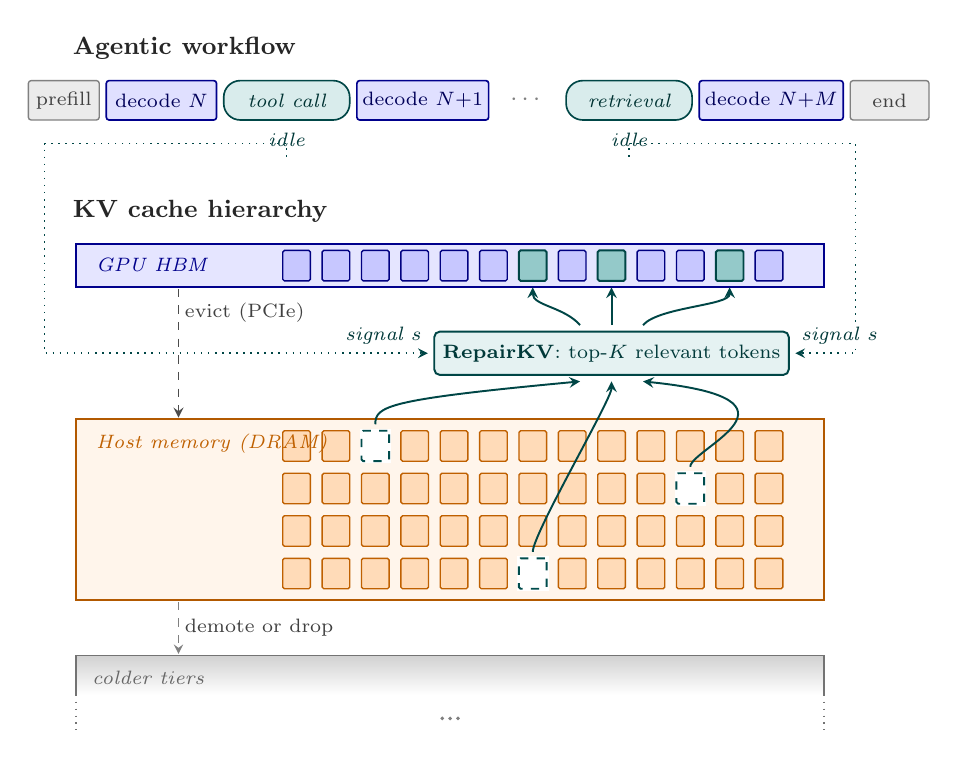
\begin{tikzpicture}[
  >=latex, line width=0.4pt, font=\small,
  % --- shared box / arrow / label styles ---
  active/.style={draw=blue!55!black, fill=blue!10, line width=0.6pt,
                 inner sep=2pt},
  store/.style={draw=orange!70!black, fill=orange!8, line width=0.6pt,
                inner sep=2pt},
  groupbox/.style={draw=orange!55, dashed, line width=0.5pt, rounded corners=2pt},
  grouplabel/.style={font=\scriptsize\itshape, text=orange!75!black},
  rowlabel/.style={font=\itshape\scriptsize},
  arrlabel/.style={font=\scriptsize, text=black!75, fill=white, inner sep=1pt},
  panellabel/.style={font=\bfseries, text=black!85},
  % --- chip styles (uniform across active and host) ---
  chip/.style={rounded corners=0.6pt, minimum width=10pt, minimum height=11pt,
               inner sep=0pt, line width=0.5pt},
  gpuchip/.style={chip, draw=blue!50!black, fill=blue!22},
  hostchip/.style={chip, draw=orange!75!black, fill=orange!28},
  promchip/.style={chip, draw=teal!55!black, fill=teal!42, line width=0.7pt},
  ghostchip/.style={chip, draw=teal!60!black, fill=white, dashed, line width=0.7pt},
  % --- timeline event pills ---
  evprefill/.style={draw=black!50, fill=black!8, line width=0.5pt,
                    rounded corners=1pt, minimum height=0.50cm,
                    inner sep=2pt, align=center, font=\scriptsize, text=black!75},
  evdecode/.style={draw=blue!55!black, fill=blue!12, line width=0.6pt,
                   rounded corners=1pt, minimum height=0.50cm,
                   inner sep=2pt, align=center, font=\scriptsize, text=blue!35!black},
  evidle/.style={draw=teal!55!black, fill=teal!15, line width=0.6pt,
                 rounded corners=6pt, minimum height=0.50cm,
                 inner sep=2pt, align=center,
                 font=\scriptsize\itshape, text=teal!40!black},
  callout/.style={font=\scriptsize, text=teal!40!black, align=center},
  % --- arrows ---
  evictarr/.style={->, line width=0.6pt, draw=black!70, dashed, >=stealth},
  promarr/.style={->, line width=1.2pt, draw=teal!55!black, >=stealth},
  faint/.style={->, line width=0.4pt, draw=black!35, >=stealth},
  arr/.style={->, line width=0.55pt, draw=black, >=stealth}
]

% =====================================================================
% LAYOUT — y-coords (top to bottom, large y = up):
%   (a) timeline:   y in [4.55, 6.55]   ~2 cm tall
%   (b) tiered+chips: y in [0.10, 4.10] ~3.0 cm tall
% Shared horizontal extent: x in [0, 13]. Panel labels at x = -0.5.
% =====================================================================
\def\xLab{-0.5}
\def\xL{0.10}
\def\xR{13.00}

% =====================================================================
% Panel (a) — Activity timeline (workflow strip + |C| polyline)
% =====================================================================
% Single combined figure (no (a)/(b) split — they interact).

% Section header: Agentic workflow — fixed gap of 0.15cm above workflow strip
% Workflow strip top at evY + evtH/2 = 5.95 + 0.25 = 6.20 → baseline 6.35.
\def\labelX{0.55}
\node[font=\bfseries\small, text=black!85, anchor=south west]
     at (\labelX, 6.35) {Agentic workflow};

% --- workflow event row ---
\def\evY{5.95}
\node[evprefill, minimum width=0.9cm, anchor=west] (evP)  at (\xL,\evY) {prefill};
\node[evdecode,  minimum width=1.4cm, anchor=west, right=2pt of evP]  (evD1) {decode~$N$};
\node[evidle,    minimum width=1.6cm, anchor=west, right=2pt of evD1] (evI1) {tool call};
\node[evdecode,  minimum width=1.6cm, anchor=west, right=2pt of evI1] (evD2) {decode~$N{+}1$};
\node[anchor=west, font=\small, text=black!50, right=4pt of evD2] (evDots) {$\cdots$};
\node[evidle,    minimum width=1.6cm, anchor=west, right=4pt of evDots] (evI2) {retrieval};
\node[evdecode,  minimum width=1.6cm, anchor=west, right=2pt of evI2] (evD3) {decode~$N{+}M$};
\node[evprefill, minimum width=1.0cm, anchor=west, right=2pt of evD3] (evEnd) {end};

% Small italic "idle" labels below each teal pause pill — the SOURCE of the
% "execute on extracted signal s" arrows.
\node[font=\itshape\scriptsize, text=teal!45!black, anchor=north]
     (idleA) at ([yshift=-1pt]evI1.south) {idle};
\node[font=\itshape\scriptsize, text=teal!45!black, anchor=north]
     (idleB) at ([yshift=-1pt]evI2.south) {idle};

% (|C| polyline dropped — workflow strip alone above)

% Section header: KV cache hierarchy — same font, same x, same gap-from-block as Agentic workflow.
% Active strip top at 3.85 + 0.275 = 4.125; gap = 0.15 → baseline 4.275.
% Lowered further so the gap to the detour horizontal at y=5.40 is ~0.925cm
% (roughly double the prior ~0.475cm).
\node[font=\bfseries\small, text=black!85, anchor=south west]
     at (\labelX, 4.275) {KV cache hierarchy};

% Geometry: CENTER-aligned tier boxes — workflow centered ON box midpoint so that
% (boxLeft - prefill_left) = (workflow_right - boxRight); both sides jut symmetrically.
\def\boxW{9.50}                 % shared visual width across tiers
\pgfmathsetmacro{\boxCx}{(\xL + 10.83)/2}     % workflow ends at evEnd.east ~ 10.83
\pgfmathsetmacro{\boxLeft}{\boxCx - \boxW/2}

% --- Active strip (THIN, single row of 13 chips) — entire KV-cache region
% shifted down a further 0.45cm (cumulative ~0.65cm) to roughly DOUBLE the
% breathing band between Agentic workflow and the KV cache hierarchy header.
\def\actY{3.85}
\def\actH{0.55}
\node[active, minimum width=\boxW cm, minimum height=\actH cm, anchor=center]
     (actBox) at (\boxCx, \actY) {};

% Place 13 chips in active: 10 blue + 3 teal SCATTERED at cols 7, 9, 12
% (mirrors the host scatter pattern; promoted tokens slot back into their
% original sequence positions, not appended at the end).
\def\actNchips{13}
\def\actChipStep{0.50}
\pgfmathsetmacro{\actXa}{\boxLeft + 2.80}   % shifted right to clear "GPU active KV cache" label
\foreach \i in {1,2,3,4,5,6,8,10,11,13}{%
  \pgfmathsetmacro{\xc}{\actXa + (\i-1)*\actChipStep}
  \node[gpuchip] (gpuChip\i) at (\xc, \actY) {};
}
\foreach \i in {7,9,12}{%
  \pgfmathsetmacro{\xc}{\actXa + (\i-1)*\actChipStep}
  \node[promchip] (gpuChip\i) at (\xc, \actY) {};
}
% Middle teal anchor (chip 9) — RepairKV centered under this chip.
\pgfmathsetmacro{\tealClusterX}{\actXa + 8*\actChipStep}

% Single tier label INSIDE active strip top-left
\node[font=\itshape\scriptsize, text=blue!55!black, anchor=north west]
     at ([xshift=4pt, yshift=-2pt]actBox.north west) {GPU HBM};

% --- Host box (LARGE 2D grid: 4 rows x 12 cols = 48 slots) ---
\def\hostY{0.75}
\def\hostH{2.30}
\node[store, minimum width=\boxW cm, minimum height=\hostH cm, anchor=center]
     (hostBox) at (\boxCx, \hostY) {};

\def\hostRows{4}
\def\hostCols{13}
\def\hostRowStep{0.54}                 % chosen so vertical gap ≈ horizontal gap (~0.15cm)
\def\hostColStep{0.50}                 % match GPU active so columns line up
\pgfmathsetmacro{\hostGridW}{(\hostCols - 1) * \hostColStep}
\pgfmathsetmacro{\hostXa}{\actXa}      % start at SAME x as GPU active chip 1
% Top row y, then walking down
\pgfmathsetmacro{\hostYra}{\hostY + 1.5*\hostRowStep}
\pgfmathsetmacro{\hostYrb}{\hostY + 0.5*\hostRowStep}
\pgfmathsetmacro{\hostYrc}{\hostY - 0.5*\hostRowStep}
\pgfmathsetmacro{\hostYrd}{\hostY - 1.5*\hostRowStep}

% Fill 4x13=52 positions with hostchip, then 3 scattered ghost slots
\foreach \yr in {\hostYra, \hostYrb, \hostYrc, \hostYrd}{%
  \foreach \i in {1,...,13}{%
    \pgfmathsetmacro{\xc}{\hostXa + (\i-1)*\hostColStep}
    \node[hostchip] at (\xc, \yr) {};
  }
}
% Scattered ghost slots at (col 3, row a), (col 11, row b), (col 7, row d)
\pgfmathsetmacro{\gxA}{\hostXa + 2*\hostColStep}
\pgfmathsetmacro{\gxB}{\hostXa + 10*\hostColStep}
\pgfmathsetmacro{\gxC}{\hostXa + 6*\hostColStep}
\fill[white] (\gxA - 0.20, \hostYra - 0.22) rectangle (\gxA + 0.20, \hostYra + 0.22);
\fill[white] (\gxB - 0.20, \hostYrb - 0.22) rectangle (\gxB + 0.20, \hostYrb + 0.22);
\fill[white] (\gxC - 0.20, \hostYrd - 0.22) rectangle (\gxC + 0.20, \hostYrd + 0.22);
\node[ghostchip] (ghostA) at (\gxA, \hostYra) {};
\node[ghostchip] (ghostB) at (\gxB, \hostYrb) {};
\node[ghostchip] (ghostC) at (\gxC, \hostYrd) {};

% Single tier label INSIDE host box top-left
\node[font=\itshape\scriptsize, text=orange!75!black, anchor=north west]
     at ([xshift=4pt, yshift=-2pt]hostBox.north west) {Host memory (DRAM)};

% --- evict arrow (DOWN, dashed, LEFT side) — labels TIGHT against active.south
%     so the detour horizontal arrow at midY doesn't clash.
\pgfmathsetmacro{\evictX}{\boxLeft + 1.30}
\pgfmathsetmacro{\midY}{(\actY - \actH/2 + \hostY + \hostH/2)/2}
\draw[evictarr]
     (\evictX, \actY - \actH/2 - 0.02)
     -- (\evictX, \hostY + \hostH/2 + 0.02);
\node[arrlabel, anchor=west]
     at (\evictX + 0.04, \actY - \actH/2 - 0.32) {evict (PCIe)};

% --- RepairKV mid-section: positioned directly beneath the MIDDLE teal chip
%     so the output arrow is a clean straight vertical line.
\pgfmathsetmacro{\rkvBoxX}{\tealClusterX}
\node[draw=teal!55!black, fill=teal!10, line width=0.7pt, rounded corners=2pt,
      inner sep=3pt, font=\scriptsize, text=teal!45!black, align=center,
      minimum width=2.6cm, minimum height=0.55cm]
     (rkvMid) at (\rkvBoxX, \midY) {\textbf{\repairkv{}}: top-$K$ relevant tokens};

% Three CURVED input arrows from host ghost slots UP into RepairKV mid-section
\draw[promarr, line width=0.7pt]
     ([yshift=2pt]ghostA.north)
     .. controls ([yshift=0.3cm]ghostA.north) and ([xshift=-0.6cm, yshift=-0.3cm]rkvMid.south west) ..
     ([xshift=-0.4cm, yshift=-2pt]rkvMid.south);
\draw[promarr, line width=0.7pt]
     ([yshift=2pt]ghostB.north)
     .. controls ([yshift=0.3cm]ghostB.north) and ([xshift=0.4cm, yshift=-0.3cm]rkvMid.south east) ..
     ([xshift=0.4cm, yshift=-2pt]rkvMid.south);
\draw[promarr, line width=0.7pt]
     ([yshift=2pt]ghostC.north)
     .. controls ([yshift=0.3cm]ghostC.north) and ([yshift=-0.3cm]rkvMid.south) ..
     ([yshift=-2pt]rkvMid.south);

% Three curved output arrows from RepairKV.north UP into the 3 SCATTERED teal
% chips at cols 7, 9, 12. Mirrors the 3 input arrows from host ghost slots.
\draw[promarr, line width=0.7pt]
     ([xshift=-0.4cm, yshift=2pt]rkvMid.north)
     .. controls ([xshift=-0.6cm, yshift=0.3cm]rkvMid.north) and ([yshift=-0.3cm]gpuChip7.south) ..
     ([yshift=-2pt]gpuChip7.south);
\draw[promarr, line width=0.7pt]
     ([yshift=2pt]rkvMid.north) -- ([yshift=-2pt]gpuChip9.south);
\draw[promarr, line width=0.7pt]
     ([xshift=0.4cm, yshift=2pt]rkvMid.north)
     .. controls ([xshift=0.6cm, yshift=0.3cm]rkvMid.north) and ([yshift=-0.3cm]gpuChip12.south) ..
     ([yshift=-2pt]gpuChip12.south);

% --- "execute on extracted signal s" — two TEAL DOTTED arrows originating
%     FROM the idle labels (not from the pills themselves), routed AROUND
%     the GPU active strip via L-shape detours.
\pgfmathsetmacro{\detourLX}{\boxLeft - 0.40}
\pgfmathsetmacro{\detourRX}{\boxLeft + \boxW + 0.40}

% Tool call (left) detour: idle label -> down -> horizontal left -> down -> right into RepairKV.west
% Horizontal segment at y = 5.40 — clean right-angle path (V-then-H) so there is no
% diagonal kink and the horizontal sits above the KV-cache-hierarchy label (top ~4.825).
\draw[->, line width=0.55pt, draw=teal!55!black, dotted, >=stealth]
     (idleA.south) |- (\detourLX, 5.40)
     -- (\detourLX, \midY)
     -- ([xshift=-2pt]rkvMid.west);

% Retrieval (right) detour: mirror on the right
\draw[->, line width=0.55pt, draw=teal!55!black, dotted, >=stealth]
     (idleB.south) |- (\detourRX, 5.40)
     -- (\detourRX, \midY)
     -- ([xshift=2pt]rkvMid.east);

% "signal s" labels: SYMMETRIC around RepairKV, sitting just outside each side
% of the pill, ABOVE the lower horizontal detour line entering RepairKV.
\node[font=\itshape\scriptsize, text=teal!45!black, anchor=south east,
      fill=white, inner sep=1pt]
     at ([xshift=-3pt, yshift=2pt]rkvMid.west) {signal $s$};
\node[font=\itshape\scriptsize, text=teal!45!black, anchor=south west,
      fill=white, inner sep=1pt]
     at ([xshift=3pt, yshift=2pt]rkvMid.east) {signal $s$};

% (label "execute on extracted signal s" removed — arrows speak for themselves)

% --- Colder tiers — open-bottom rectangle with dotted side extensions ---
\def\coldYtop{-1.10}
\def\coldYbot{-1.60}
\pgfmathsetmacro{\coldL}{\boxLeft}
\pgfmathsetmacro{\coldR}{\boxLeft + \boxW}
% Light grey fill that fades from top (more visible) to bottom (faint)
\shade[top color=black!18, bottom color=white]
     (\coldL, \coldYbot) rectangle (\coldR, \coldYtop);
% Top edge (solid)
\draw[draw=black!55, line width=0.6pt] (\coldL, \coldYtop) -- (\coldR, \coldYtop);
% Side edges: solid in the visible band, then dotted extensions going down
\draw[draw=black!55, line width=0.6pt] (\coldL, \coldYtop) -- (\coldL, \coldYbot);
\draw[draw=black!55, line width=0.6pt] (\coldR, \coldYtop) -- (\coldR, \coldYbot);
\draw[draw=black!55, line width=0.5pt, dotted]
     (\coldL, \coldYbot) -- (\coldL, \coldYbot - 0.45);
\draw[draw=black!55, line width=0.5pt, dotted]
     (\coldR, \coldYbot) -- (\coldR, \coldYbot - 0.45);
% Three subtle dots at the bottom-center to imply "continues"
\foreach \dx in {-0.10, 0, 0.10}{%
  \fill[black!50] ({\boxCx + \dx}, \coldYbot - 0.30) circle (0.025);
}
% Single tier label INSIDE cold tier top-left
\node[font=\itshape\scriptsize, text=black!60, anchor=north west]
     at (\coldL + 0.08, \coldYtop - 0.08) {colder tiers};

% Arrow from Host to Cold (spill, dashed, faint) — aligned with evict on left
\pgfmathsetmacro{\spillX}{\evictX}
\draw[->, line width=0.5pt, draw=black!50, dashed, >=stealth]
     (\spillX, \hostY - \hostH/2 - 0.02)
     -- (\spillX, \coldYtop + 0.02);
\node[arrlabel, anchor=west]
     at (\spillX + 0.04, {(\hostY - \hostH/2 + \coldYtop)/2}) {demote or drop};

\end{tikzpicture}
\end{document}
